%% content.tex
%%


%% ===========================
\chapter{Umsetzung}
\label{ch:umsetzung}
%% ===========================


%% ===========================
\section{Aufbau der Server.war}
%% ===========================

Die Web-Archive-Datei beinhaltet ein dynamisches Web-Projekt aus dem Eclipse Web Tools Platform (WTP) Projekt. Aufgrund der typischen Struktur des Web-Projekts, wird im folgenden nur auf die Klassen eingegangen. Abbildung \ref{umsetzung_klassendiagramm_server} zeigt das Klassendiagramm der Server.war. Das Diagramm dient als Basis für die nachfolgenden Erläuterungen. 

Die H2-Datenbank wird im Embedded-Modus betrieben, was eine Instanziierung der Datenbank zur Laufzeit notwendig macht. Die Instanziierung erfolgt in der Klasse Database. Das Attribut dataSource stellt die H2-Datenbank in Form eines Objektes dar. Eine Verbindung zur Datenbank wird mithilfe der Methode .getConnection() aufgebaut. Diese Verbindung wird permanent offen gehalten, solang der Tomcat Server läuft. Dazu wird die Verbindung dem Attribut con zugewiesen, die von allen Methoden verwendet wird die eine Verbindung zur Datenbank aufbauen wollen. Um die Datenbank mit der Web-Anwendungen zu starten, ist die Verwendung eines Servlets nötig. Dazu benutzen wir die Klasse EntryPoint die das Interface HttpServlet implementiert. Um das Servlet direkt beim Start aufzurufen wird in der web.xml folgende Zeilen eingetragen: 

\begin{lstlisting}[language=XML]
	<servlet>
		<servlet-name>H2</servlet-name>
		<servlet-class>de.cas.db.EntryPoint</servlet-class>
		<load-on-startup>1</load-on-startup>
	</servlet>
\end{lstlisting}

Die 1 im Element <load-on-startup> bewirkt den Aufruf der Methode init() die eine Instanziierung der Klasse Database vornimmt. Zur Erzeugung des Schemas wird eine separate Klasse namens SchemaBuilder eingesetzt. In Ihr werden sämtliche SQL-Anweisungen zur Generierung des Schemas aufbewahrt und können über die Methode createSchema() ausgeführt werden.

Mit der Klasse JerseyServer wird der REST-Server umgesetzt. Sie besitzt Methoden die mit den entsprechenden Annotationen, wie @GET oder @POST, die REST-Requests entgegen nehmen. Mit der Annotation @Path wird die URL angegeben, unter der die Methode angesprochen werden kann. Diese Methoden können Übergabeparameter vom Typ UriInfo und/oder HttpHeaders besitzen, die Abrufe von Metadaten der REST-Requests ermöglichen. 

\begin{figure}[htbp]
\begin{center}
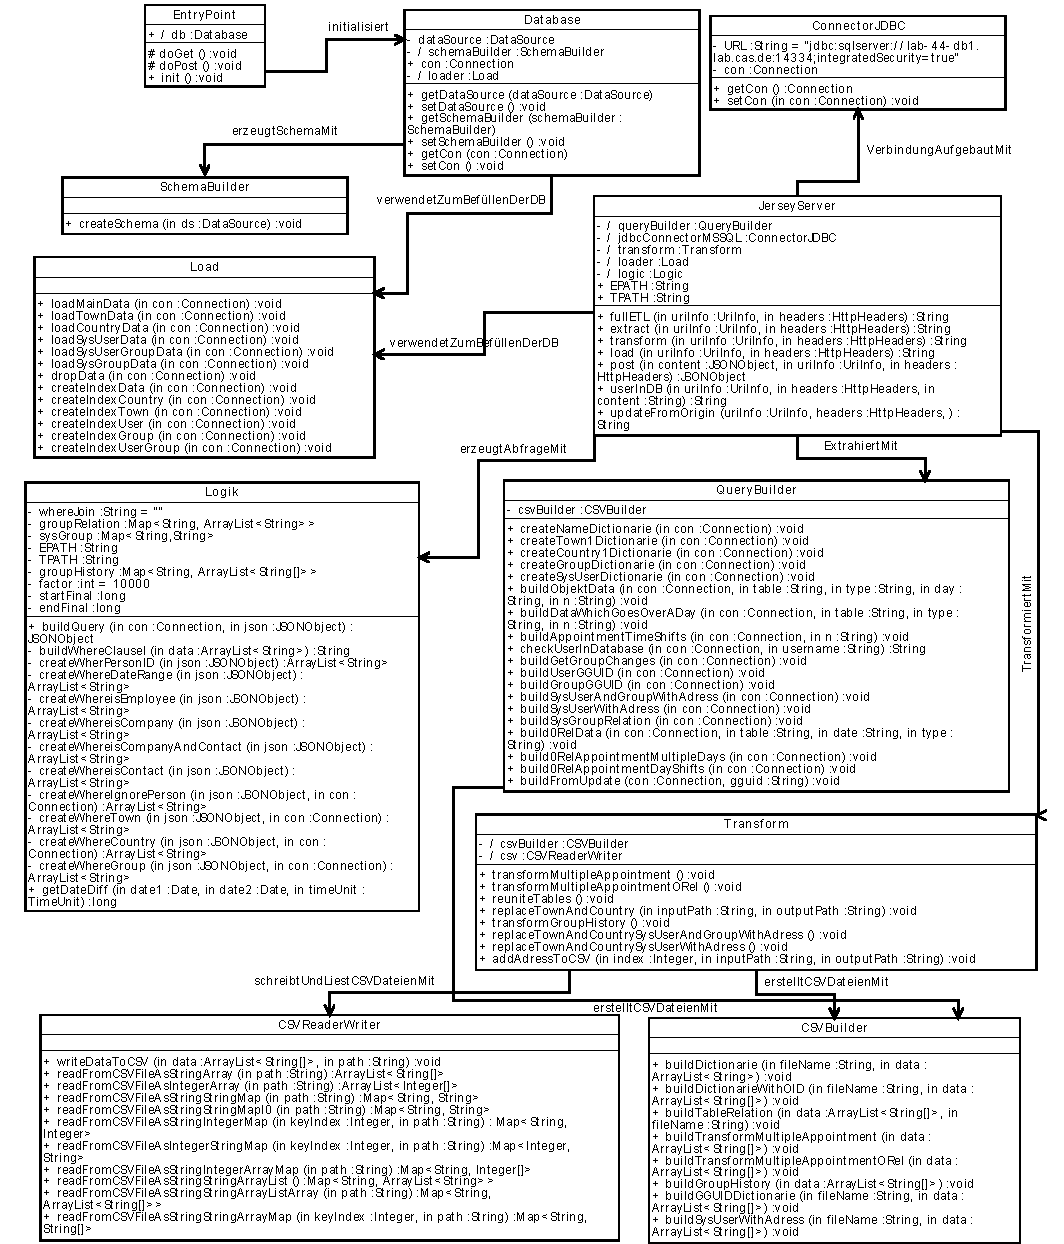
\includegraphics[width=1.0\textwidth]{pics/ServerKlassendiagramm.pdf}
\caption{Server Klassendiagramm}
\label{umsetzung_klassendiagramm_server}
\end{center}
\end{figure}

Neben den Methoden zu Beantwortung von REST-Requests, enthält die Klasse alle Objekte zur Durchführung des ETL-Prozesses. Die Klasse ConnectorJDBC besitzt ein Attribut namens con, welches den Verbindungsaufbau zum MSSQL Server, mithilfe von JDBC ermöglicht. Zur Extraktion der Daten aus dem MSSQL Server, wird ein Objekt der Klasse QueryBuilder verwendet. Wie in der Abbildung zu sehen, werden für die verschiedenen Tabellen des neuen Schemas, eigene Methoden zur Verfügung gestellt. Methoden welche die Übergabewerte table, date und n besitzen, werden für die verschiedenen Verbindungsmerkmale benötigt. Mithilfe des Parameters table, wird der Name der Tabelle in der MSSQL Datenbank übergeben. Der Parameter date gibt das Feld an, was für die Ermittlung des Datums verwendet werden soll. Um den Typ eines Verbindungsmerkmals zwischen Personen festzuhalten, wird der Parameter n verwendet, der eine Zahl zwischen eins und fünf beinhaltet. QueryBuilder verwendet ein Objekt vom Typ CSV-Builder, um die Ergebnisse in Dateien festzuhalten. Den Methoden wird als Übergabeparameter ein Dateiname, sowie die Daten selbst übergeben.

Die Klasse Transform enthält Attribute und Methoden zur Bearbeitung der CSV-Dateien. Weiterhin werden, die durch die Extraktionen gewonnen CSV-Dateien, mithilfe eines CSVReaderWriter Objekts ausgelesen. Nach der Bearbeitung durch die Methoden der Transform-Klasse, werden die Daten wieder in CSV-Dateien abgelegt. CSVBuilder besitzt Methoden die zusätzliche Parameter zum schreiben aufweisen, die modifizierte Schreiboperationen erlauben. Wohingegen CSVReaderWriter mithilfe der Methode writeDataToCSV(), sowie den Parametern path und data allgemeine Schreiboperationen durchführt.

Mithilfe der Klasse Load, wird die Datenbank befüllt. Sie kann wie zuvor erwähnt, von einem Database Objekt verwendet werden oder durch ein JerseyServer Objekt. Beim JerseyServer werden mit der Methode load(), die Methoden der Load-Klasse aufgerufen. In der Klasse Database werden sie im Konstruktor aufgerufen. 

Die Logik Klasse enthält alle Attribute und Methoden, zur Beantwortung von Anfragen, durch den Nutzer. Zur Generierung der Bedingungen einer SQL-Abfrage, werden separate Methoden verwendet. Die jeweiligen Methoden werden nur gerufen, sobald die entsprechende Bedingung, in der vom Nutzer erhaltenen JSON Datei, vorhanden ist. Angesteuert wird der Bau einer Abfrage durch die Methode buildQuery(). 

%% ===========================
\section{Aufbau der Client.war}
\label{ch:Umsetzung:sec:clientwar}
%% ===========================

\begin{figure}[htbp]
\begin{center}
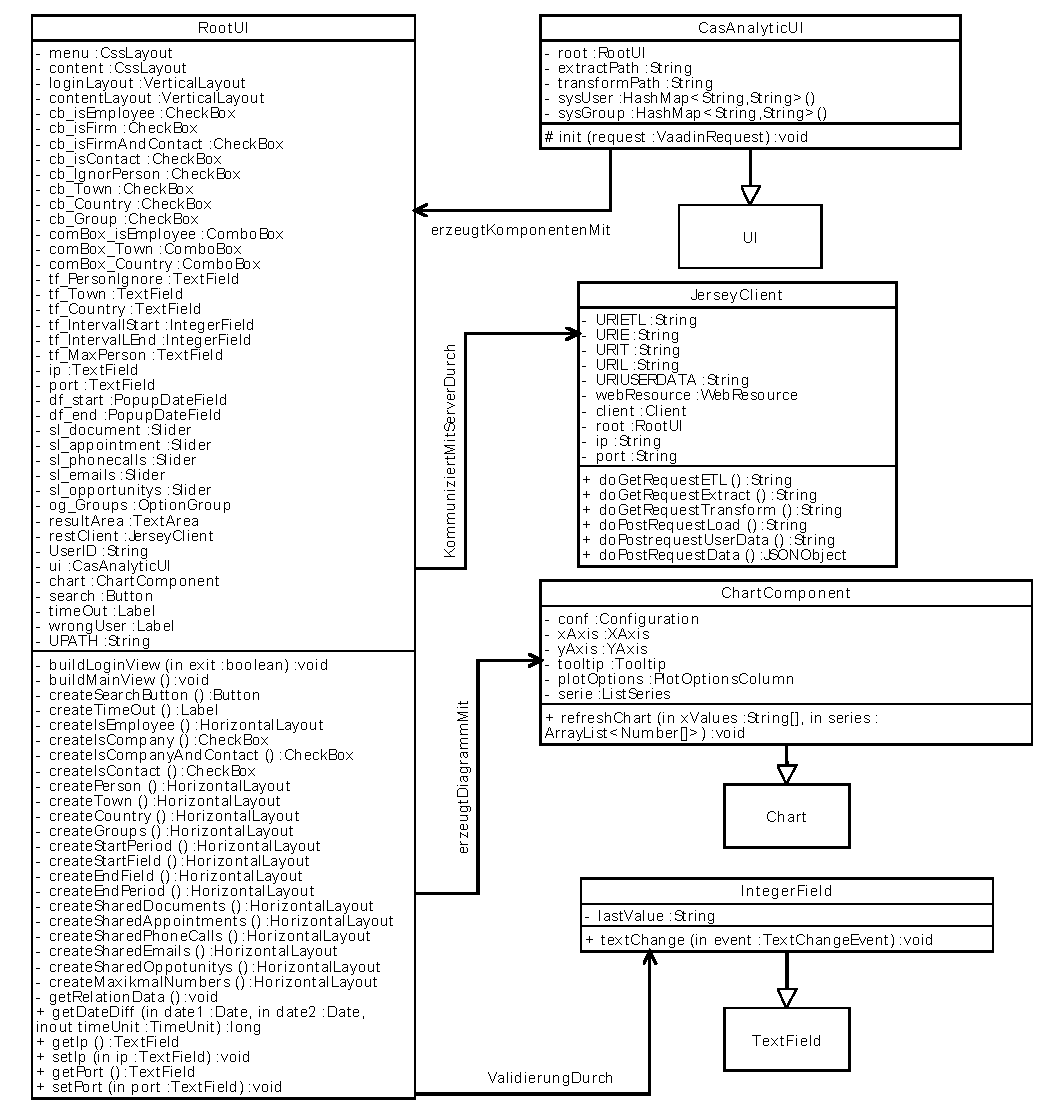
\includegraphics[width=1.0\textwidth]{pics/ClientKlassendiagramm.pdf}
\caption{Client Klassendiagramm}
\label{umsetzung_klassendiagramm_client}
\end{center}
\end{figure}

Einstiegspunkt in der Client.war ist die Klasse CasAnalyticUI. Sie ist von der Klasse UI abgeleitet. Die UI ist die oberste Komponente jeder Komponentenhierarchie. Es gibt eine Benutzeroberfläche für jede Vaadin-Instanz in einem Browser-Fenster. Ein UI Objekt kann entweder ein gesamtes Browser-Fenster (oder Tab) oder einen Teil einer HTML-Seite, wo eine Vaadin-Anwendung eingebettet ist, darstellen. Nachdem eine UI von der Anwendung erstellt wurde, wird es mit der Methode init(VaadinRequest) initialisiert. Zur Übersicht werden die Komponenten der Darstellung in die Klasse RootUI ausgelagert. 

RootUI wird dabei von der CasAnalayticUI instanziiert. Die Klasse RootUI beinhaltet das Anmeldefenster, sowie die Hauptansicht. Mithilfe der Methode buildLoginView() werden die Komponenten des Anmeldefensters zur UI hinzugefügt. Nach der Erzeugung der Komponenten, wird eine JerseyClient Klasse instanziiert. Diese wird verwendet sobald der Nutzer IP, Port und einen Namen eingegeben hat und auf anmelden geklickt hat. Anschließend wird die Methode doPostRequestUserData() gerufen, um zu überprüfen ob der Nutzer im System existiert. 

Falls ja werden durch die Methode MainView() alle bisherigen Komponenten der UI entfernt und durch Komponenten des Hauptfensters ersetzt. Das JerseyClient Objekt wird direkt im Anschluss verwendet, um Mithilfe der Methode doPostRequestData() einen REST-Request an den Server zu senden. Dieser liefert das Ergebnis der Abfrage in einem JSON-Objekt zurück. Mit dessen eine erste Darstellung der Diagramms erzeugt wird. Das Diagramm selbst besitzt eine eigene Klasse namens ChartComponent. Sie leitet sich von der Klasse Chart ab, die Teil der VaadinChart Bibliothek ist. Mithilfe der Methode refreshChart() wird das Diagramm bei Benutzerabfragen aktualisiert. Dazu werden ihr die Namen der Personen für die x-Achse übergeben, sowie die neuen Balkenwerte. Weiterhin wird für jedes Vaadin-Objekt das eine Element an der Oberfläche darstellt, eine separate Methode zur Erzeugung verwendet. Änderungen am Aussehen oder der Funktion, der jeweiligen Vaadin-Objekte, werden nur innerhalb der entsprechenden Methode vorgenommen.

An der Oberfläche gibt es Felder die nur Zahlen erwarten. Eingaben die nicht numerisch sind, werden durch den Einsatz der Klasse IntegerField verhindert. Diese erweitert die Klasse TextField. Sie besitzt einen Event-Listener, der jede Eingabe des Benutzers abfängt. Gibt der Nutzer nicht numerische Zeichen ein werden diese direkt wieder entfernt. Dadurch werden falsch Eingaben durch den Nutzer ausgeschlossen.

%% ===========================
\section{Erzeugung der Abfrage}
%% ===========================

Um Abfragen durch den Benutzer möglichst performant zu beantworten erfolgt die Erzeugung dynamisch. Das bedeutet die SQL-Abfrage an die Datenbank kann je nach Anforderung anders aufgebaut sein. Die Kernaufgabe ändert sich jedoch nie. Diese besteht aus der Bildung von Summen basierend auf verschiedenen Verbindungsmerkmalen. Zu Berücksichtigen ist das jede Abfrage einen Anfangs- und Endzeitpunkt enthält und somit beachtet werden muss. Nachdem festgestellt wurde wie viele Verbindungsmerkmale von den jeweiligen Typen zu einer Person verlaufen wird zusätzlich die Gesamtsumme der Verbindungsmerkmale zu einer Person gebildet. Die Summe wird zur Sortierung der Ergebnisse verwendet. Bei der Sortierung wird absteigend vorgegangen, um die Personen mit den meisten Verbindungsmerkmale zu der von der Suche ausgehend Person zu ermitteln. Das Ergebnis wird wiederum auf eine durch den Benutzer festgelegte Anzahl reduziert. 

Zu diesen Kernfunktionalitäten können durch Angaben des Nutzers weitere hinzukommen. Eine von Ihnen ist die Gewichtung von Zeitpunkten. Der Ansatz zur Umsetzung der Gewichtung der Zeit wird anhand der Abbildung \ref{fig:umsetzung:gewichtungderzeit} erklärt. Die Abbildung zeigt ein Koordinatensystem mit den Gewichtung von einzelnen Zeitpunkten. Die x-Achse stellt den zeitlichen Verlauf dar. Während die y-Achse die Gewichtung darstellt. $t_{start}$ markiert den Startzeitpunkt, wohingegen $t_{end}$ den Endzeitpunkt angibt. Mithilfe von $t_1$ und $t_2$ werden Zeitspannen festgelegt, die differenziert zu gewichten sind. Um nun die Tage zu gewichten wurde der lineare Ansatz gewählt. Das bedeutet zwischen $t_{start}$ und $t_1$ steigt die Relevanz stetig bis sie die 100 Prozent erreicht hat. Ab dort sind alle Tage wieder 100 Prozent relevant außer es ist ein $t_2$ angegeben worden. Falls ja wird ab $t_2$ linear fallend, jeder Tag bewertet. 

Zur Berechnung der Gewichtung zu einem bestimmten Tag werden die folgenden zwei Variablen verwenden:

\begin{equation}
f_1 = \frac{1}{t_1 - t_{start}}
\end{equation}
\begin{equation}
f_2 = \frac{1}{t_{end} - t_2}
\end{equation}

Dabei wird wie folgt vorgegangen. $t_{start}$ markiert Tag. Aufsteigend zählend wird jeder Tag bis $t_1$ mit der Variabel $f_1$ multipliziert. Für den Zeitpunkt $t_2$ wird die Summe der Tage in der Zeitspanne zwischen $t_2$ und $t_{end}$ verwendet. Die Summe wird mit jedem weiteren Tag um 1 vermindert bis zum Zeitpunkt $t_{end}$, der 0 darstellt. Bei jedem Schritt wird der Tag mit der Variablen $f_2$ multipliziert.

\begin{figure}[htbp]
\begin{center}
\begin{tikzpicture}[domain=-1:2] \draw[very thin,color=gray] (0,0); 
\draw[->] (0,0) -- (12.3,0) node[right] {Zeit}; 
\draw[->] (0,0) -- (0,4.2) node[above] {Faktor Gewichtung}; 
\draw[color=black]  (0.2,3) -- (-0.2,3)   node[left] {100\%};
\draw[color=black]  (0.2,1.5) -- (-0.2,1.5)   node[left] {50\%};  
\draw[dashed][color=black]  (5,0.5) -- (5,3.5); 
\draw[dashed][color=black]  (9,0.5) -- (9,3.5);

\draw[color=black]  (0,0) -- (0,0)   node[below] {$t_{start}$}; 
\draw[color=black]  (5,0.1) -- (5,-0.1)   node[below] {$t_1$}; 
\draw[color=black]  (9,0.1) -- (9,-0.1)   node[below] {$t_2$};
\draw[color=black]  (12,0.1) -- (12,-0.1)   node[below] {$t_{end}$};   
 
\draw[color=black]  (0,0) -- (5,3)   node[right] {}; 
\draw[color=black]  (5,3) -- (9,3)   node[right] {}; 
\draw[color=black]  (9,3) -- (12,0)   node[right] {};  

\end{tikzpicture} 
\end{center}
\caption{Gewichtung der Zeit}
\label{fig:umsetzung:gewichtungderzeit}
\end{figure}

Neben der Gewichtung der Zeit lassen sich die jeweiligen Verbindungsmerkmale unterschiedlich gewichten. Bei einer Abweichung von 100 Prozent wird die Summe des jeweiligen Verbindungsmerkmales, um die durch den Nutzer bestimmten Prozentsatz verringert. 

Die restlichen Parameter dienen der Filterungen und werden je nach Nutzer-Eingabe, zu den Bedingungen der SQL-Abfrage hinzugenommen. Unter Ihnen gibt es eine Bedingung, die zuvor ermittelt werden muss und daher näher beschrieben wird. Dabei handelt es sich um die Ausschluss von Gruppen, da sich ihre Zusammensetzung über die Zeit variabel ist. Dazu wird die Tabelle UserGroup verwendet. Dabei wird wie folgendermaßen vorgegangen. Zuerst wird die Ergebnismenge auf die ausgewählten Gruppen reduziert. Anschließend wird für jede Gruppe ein eigener Container erzeugt, der alle Personen der Gruppe enthält. Liegt nun das Feld Date nach dem Anfangszeitpunkt der Abfrage und die Spalte Action enthält eine 1, wird der Container um diese Person reduziert. Enthält die Spalte Action eine 0 wird die Person zum Container hinzugefügt. Die 1 in der Spalte Action bedeutet das die Person zu dem in der Spalte Date angegeben Datum die Gruppe verlassen hat. Eine 0 bedeutet das die Person zu dem angegeben Datum hinzukam. Dadurch wird die Zusammensetzung zum Anfangszeitpunkt wiederhergestellt. Mithilfe der Personen aus den Container wird nun die SQL-Abfrage um weitere Bedingungen erweitert.

Zu beachten ist natürlich das innerhalb des Zeitraums Gruppenveränderungen stattgefunden haben können, diese jedoch nicht zu Berücksichtigen sind. Es kann jeweils nur ein bestimmter Zeitpunkt für die Betrachtung berücksichtigt werden. In diesem Fall wurde der Anfangszeitpunkt gewählt.

%% ===========================
\section{ETL Prozess}
%% ===========================

Um an die notwendigen Daten zu gelangen werden zuerst die Informationen aus der alten Datenbank extrahiert. Dazu wird ein Verbund gebildet der die Tupeln der Tabellen verschmelzen lässt. Die manuellen erstellten Verbindungen in der alten Datenbank werden mithilfe der Tabelle TableRelation festgehalten. Zur Gewinnung dieser Verbindungen wird als erstes eine SQL-Abfrage definiert die für jede der Tabellen gwOpportunity, gwPhoneCall0, Document0, EmailStore0 und Appointment0 separat ausgeführt wird. 

Mithilfe des ersten Verbundes zwischen SysUser und Adresse wird die Adresse einer Person ermittelt. Anschließend wird durch einen Verbund der TableRelation und SysUser alle Tabellen ermittelt die mit der Person eine Verbindung besitzen. Der nächste Verbund ist zwischen TableRealtion und einer der fünf zuvor genannten Tabellen. Um festzustellen welche Personen auch mit beispielsweise einem Dokument arbeiten zu ermitteln wird ein weiterer Verbund mit der passenden ORel-Tabelle ausgeführt. In der ORel-Tabelle kann die OID positiv sowie negativ sein. Bei einem negativen Wert stellt die OID eine GID der Tabelle SysGroup dar. Zur Auflösung der Gruppe in einzelne Personen werden folgende Verbunde gebildet. Zuerst zwischen SysGroup und SysGroupMember um alle Personen die zu einer Gruppe gehören zu erhalten. Anschließend zwischen SysGroupMember und SysUser um die OID der Person zu erhalten. 

Nachdem alle Information in einem Verbund vorhanden sind werden lediglich drei Informationen des Gesamten Verbundes behalten. Zu einem die OID des SysUser von dem die Suche ausgeht. Zum anderen das Datum welches durch das Objekt welches die Personen verbindet ermittelt wird. Weiterhin wird die zweite OID durch den Verbund mit einer zweiten SysUser Tabelle behalten. Zum Schluss wird manuell eine vierte Information beigefügt die besagt welchem Objekt die Tupel entstammt. 

Für den Sonderfall das ein Datum über mehrere Tage geht wird eine fünfte Spalte hinzugefügt welche den Zeitraum in Tagen beinhaltet. Zur Beschaffung der geschobenen Termine wird genau wie in der Konzeption beschrieben verfahren.

Zur Ermittlung direkter Verbindungen zwischen Personen wird lediglich ein Verbund aus zwei ORel-Tabellen eines Objektes gebildet. Dieser Verbund beinhaltet bereits die OIDs der beiden Personen. Zur Ermittlung des Datums wird noch ein Verbund mit der Tabelle des Objektes gebildet. Die negativen OIDs werden genauso wie oben beschrieben aufgelöst. 

Jede Antwort einer SQL-Abfrage zur Gewinnung von Daten wird in einer SCV-Datei direkt auf dem Tomcat Server abgelegt. Diese CSV Dateien stellen die Grundlage der Transformation dar. Jede dieser Dateien beinhaltet Verbindungen zwischen Personen in der Form wie sie Abbildung \ref{fig:umsetzung_csv_datei} zeigt. 

\begin{figure}[htbp]
\begin{center}
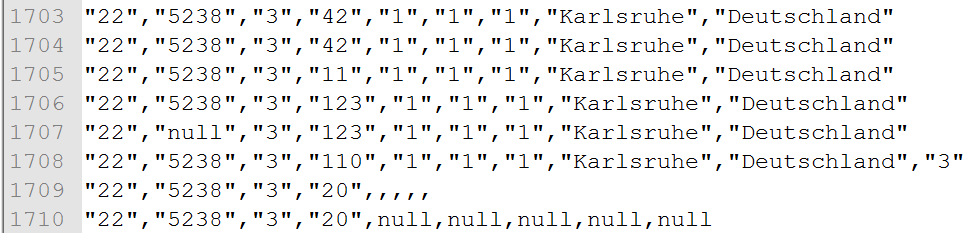
\includegraphics[width=1.0\textwidth]{pics/umsetzung_csv_datei.png}
\caption{Ausschnitt einer CSV-Datei mit Daten der Extraktion}
\label{fig:umsetzung_csv_datei}
\end{center}
\end{figure}

Alle CSV-Dateien werden auf die in Abbildung \ref{fig:umsetzung_csv_datei} zu sehenden Ungereimtheiten untersucht. Dabei werden Zeilen wo die letzten fünf Werte fehlen über die die OID (die vierte Zahl) die Adresse ergänzt. Bei null Werten wird überprüft ob wirklich keine Adresse vorhanden ist falls doch werden diese ebenfalls ergänzt. Wenn wie in Zeile 1707 zu sehen eine null Anstatt einem Datum steht wird die Zeile entfernt. Falls wie in Zeile 1708 ein zusätzlicher zehnter Wert vorhanden ist, bedeutet das die Verbindung über mehrere Tage geht. Die Zeile bleibt bestehen jedoch wird der letzte Wert entfernt. Die Zahl wird jedoch noch verwendet um die weiteren Zeilen mit aufsteigendem Datum zu erzeugen. Nach der Beseitigung von Anomalien werden noch die Städte und Länder durch ihre jeweilige ID aus der Tabelle Town und Country ersetzt.

Die veränderten Daten werden wieder in CSV-Dateien abgelegt die gleich bezeichnet sind allerdings noch den Zusatz "\_transf" besitzen der Sie als Transformiert  markiert. Diese Dateien werden anschließend in eine CSV-Datei zusammengeführt. Bei der Zusammenführung sind zum ersten mal alle Daten gleichzeitig in der Anwendung weshalb an dieser Stelle alle Duplikate beseitigt werden. Weiterhin werden die Zeilen sortiert. Dabei wird mit zwei Kriterien sortiert. Das erste Kriterium ist der Erste Wert die OID der Person von dem die Suche ausgeht. Wenn hierbei gleiche Werte verglichen werden wird das zweite Feld(Datum) herangezogen. Nachdem alle Zeilen sortiert und von Duplikaten bereinigt sind werden alle Zeilen in einer CSV-Datei abgelegt. 

Diese Datei wird bei jedem Start des Tomcats dazu verwendet einen Bulk-Load für die H2-Datenbank zu initialisieren. Nachdem die Datenbank mit Daten befüllt wurde werden abschließend die Indizes erzeugt.


%% ===========================
\section{Aktualisierung des Datenbestandes ...Progress}
%% ===========================

Wie zuvor in Abschnitt \ref{ch:Konzeption:sec:updatedatenbestand} behandelt wird die Aktualisierung unseres Datenbestandes von CAS genesisWorld angestoßen. Zur Umsetzung ist die Definition einer COM-Komponente notwendig. Dazu wird eine DLL-Datei angelegt. Diese muss Namenskonventionen einhalten. Dateien die aufgenommen werden sollen, müssen mit dem Prefix "pGSAxExtCustomServerDataPlugin" beginnen. Die DLL-Datei ist in der RegisterSDKDataPlugIns.xml hinterlegt, damit der Anwendungsserver beim Start unser Plugin findet. Weiterhin ist in der XML-Datei eine Tabelle paarweise mit einer DLL angegeben. Dadurch wird ein Plugin auf eine Datenbanktabelle registriert und bekommt alle betreffenden Änderungen mit.

Die Programmbibliothek selbst ist in Delphi realisiert. Abbildung \ref{ergebniss_plugin_klassendiagramm} zeigt die Struktur der DLL-Datei. Die Klasse selbst implementiert sechs verschiedene Schnittstellen. ComObj stellt Funktionen zur Erstellung und Bearbeitung von COM-Objekten zur Verfügung. Um Funktionalitäten von CAS genesisWorld vollständig zu Nutzen wird die ActiveX Schnittstelle benötigt. Wie bereits behandelt findet die Übertragung der Daten über das REST-Protokoll statt, wofür die idHttp Schnittstelle verwendet wird. Um Konvertierungen der vom Anwendungsserver erhaltenen Binärwerte vorzunehmen, werden die Funktionen der Schnittstellen CAS\_ToolsCOM und CAS\_VarType14Fix genutzt. Die eigentliche Kernfunktionalität, dass Abfangen der geänderten Daten, sind durch die Funktionen der IGWSDKDataPlugin Schnittstelle möglich.

Die Funktionen der Abbildung \ref{ergebniss_plugin_klassendiagramm} gehören von BeforeAddNew() bis AfterUndelete() zur IGWSDKDataPlugin Schnittstelle. Es sind zwar alle Funktionen in der DLL implementiert, allerdings werden nur die Funktionen die mit After beginnen auch mit Logik hinterlegt. Für unser System reicht es nämlich aus, über Änderungen im Nachhinein benachrichtigt zu werden. Diese Funktionen enthalten alle die gleiche Logik und unterscheiden sich lediglich in den Übergabeparameter.

Die Logik innerhalb der Funktionen sieht wie folgt aus. Eine Veränderungen der Datensätze wird vom Nutzer angestoßen. Das Plugin wird wird nach den Änderungen aufgerufen. Die entsprechende Funktion erhält die GGUID der Tupel, den Namen der Spalte, sowie die veränderten Werte. Anschließend wird überprüft ob die Änderungen für unser System von Relevanz ist. Dafür wird überprüft ob die betroffene Spalte zu den in in der ETL-Phase betroffenen Spalten gehört. Falls ja wird die aGGUID in einen String konvertiert. Weiterhin werden die Variablen einer idHttp Variable gesetzt. Dazu werden Werte wie die URI oder HTTP-Header zugewiesen. Sobald alle Daten in der idHttp Variable vorhanden sind, wird ein POST-Request an unser System übermittelt. 

Der POST-Request enthält lediglich die GGUID und die Art der Operation die auf den Daten ausgeführt wurde. Bei einem Update beispielsweise wird ein Header mit einem Key-Value wie "Operator:Update" übermittelt. In unserem Server wird lediglich überprüft ob der Wert der geändert wurde bereits existiert. Falls ja wird er gelöscht und neu beschafft. Falls nein wird er nur besorgt.


\begin{figure}[htbp]
\centering
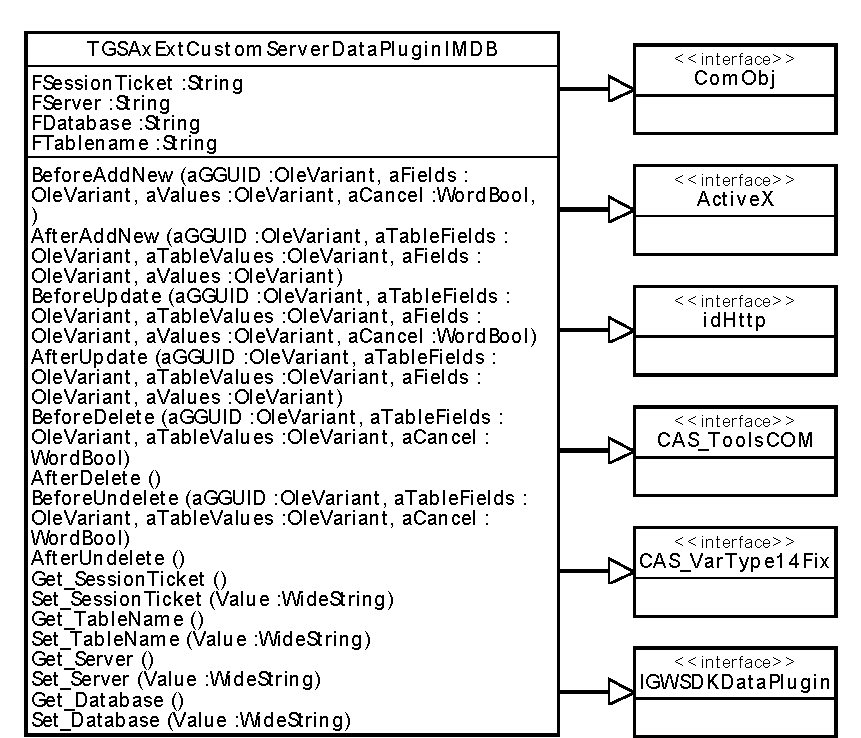
\includegraphics[scale=0.8]{pics/plugin_klassendiagramm.pdf}
\caption{Klassendiagramm Plugin}
\label{ergebniss_plugin_klassendiagramm}
\end{figure}

%% ===========================
\section{Oberfläche}
%% ===========================

In diesem Abschnitt wird die Umsetzung auf der Darstellungsebene erörtert. Den Einstiegspunkt für Nutzer stellt das in Abbildung \ref{ergebniss_oberflaeche_anmeld} zu sehende Anmeldefenster dar. Der Hintergrund der Webseite ist in einem dunklen grau Gestaltet, um sich von dem weißen Hintergrund der Bedienelemente abzuheben. Zur Identifikation des Systems mit der Firma ist dessen Logo im linken Teil dargestellt. Im rechten Teil des Fensters existieren drei Eingabefelder. Zuerst ein Feld zur Eingabe der IP-Adresse des Server. Die dazugehörige Portnummer wird im darauf folgenden Feld eingegeben. Das dritte Feld ist für den Namen des Nutzers vorgesehen, der den Ausgangspunkt der Analyse darstellt. Abschließend wird ganz klassisch ein Button zum fortfahren auf der Webseite eingesetzt. Falls allerdings der eingegeben Nutzername nicht existiert wird eine Warnmeldung direkt über dem dafür vorgesehen Feld ausgegeben. 

\begin{figure}[htbp]
\centering
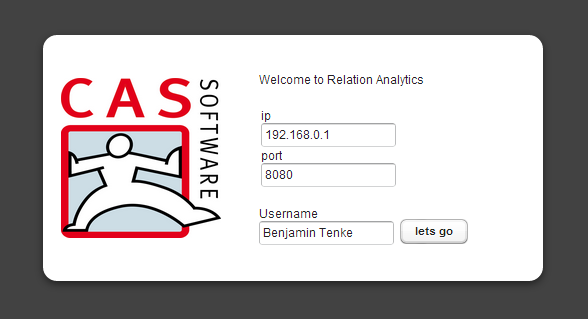
\includegraphics[scale=2.0]{pics/login.png}
\caption{Oberfläche des Systems}
\label{ergebniss_oberflaeche_anmeld}
\end{figure}

Das Hauptfenster wurde vom Aufbau wie in Abschnitt \ref{ch:Konzeption:sec:Darstellungskonzepte} beschrieben umgesetzt. Im oberen Bereich findet sich eine Leiste, die an Produkte wie Microsoft Office angelegt ist. Dies schafft ein vertrautes Gefühl mit der Oberfläche, da auf bekanntem aufgebaut werden kann. Die Leiste ist in vier Bereiche gegliedert. Der erste Bereich, ganz links, dient der Gewichtung von Suchkriterien und der Anfragestellung. Aufgrund der Gewichtung in Prozent ist ein fester Wertebereich von 0 bis 100 vorgegeben. Textfelder eignen sich daher weniger, da sie beliebige Eingaben ermöglichen. Der Einsatz von Reglern bietet eine einfachere und selbsterklärende Form der Bedienung. Der begrenzte sowie kleine Wertebereich führten zu der Entscheidung. Zum stellen der Anfrage wird ein einfacher Button eingesetzt. Direkt unter dem Button befindet sich Text, der zur Ausgabe der benötigten Zeit vorgesehen ist. 

Der zweite Bereich in der Mitte dient zeitlichen Anpassungen. Das erste und dritte Feld können zur Veränderung der Zeitspanne verwendet werden. Sie beinhalten den Anfangs- und Endzeitpunkt der Betrachtung. Händische Eingaben sind eher schlecht für die Bedienbarkeit weswegen ein sogenannter Datumspicker eingesetzt wird. Dieser befindet sich direkt neben dem Textfeld und öffnet sich nach einem klick auf das Symbol. Er stellt einen grafischen Kalender dar aus dem durch klicken auf ein Tag das Datum bestimmt werden kann. Die Möglichkeit zur Eingabe durch direktes ändern des Textes bleibt allerdings weiterhin erhalten. Die anderen beiden Felder sind für die Gewichtung der Zeit vorgesehen. In Abbildung \ref{fig:umsetzung:gewichtungderzeit} werden die Zeitpunkt bis zu dem differenziert gewichtet werden soll mit $t_1$ und $t_2$ bezeichnet. Diese Zeitpunkte können mithilfe der Textfelder bestimmt werden. Das obere Feld ist für $t_1$. Hier kann die Zeitspanne zwischen $t_{start}$ und $t_1$ in Tagen festgelegt werden. Für $t_{ende}$ und $t_2$ verhehlt es sich mit dem unteren Feld ebenso.

Bis auf die Gruppenfilterung sind im dritten Bereich alle restlichen Filtermöglichkeiten vorhanden. Mithilfe von Checkboxen kann der Nutzer festlegen welche Filterungen auf die Analyse angewendet werden sollten. Neben der Filterung durch bestimmte Personen, Länder, Städte usw. ist hier eine Begrenzung der Ergebnismenge umgesetzt. Im untersten Feld kann der Nutzer diese bestimmen.

Der Bereich ganz rechts in der Leiste ist für den Ausschluss von Gruppen vorgesehen. Hier werden alle Gruppen im System mit einer Checkbox und einem Namen dargestellt. Dabei können beliebig viele Gruppen ausgewählt werden. Da die Anzahl der Gruppen überschaubar ist entschied man sich alle anzuzeigen anstatt einer manuellen Eingabe durch den Nutzer. Das hat auch den Vorteil, dass der Benutzer Gruppen sieht die er eventuell nicht exakt beim Namen kennt.     

\begin{figure}[htbp]
\centering
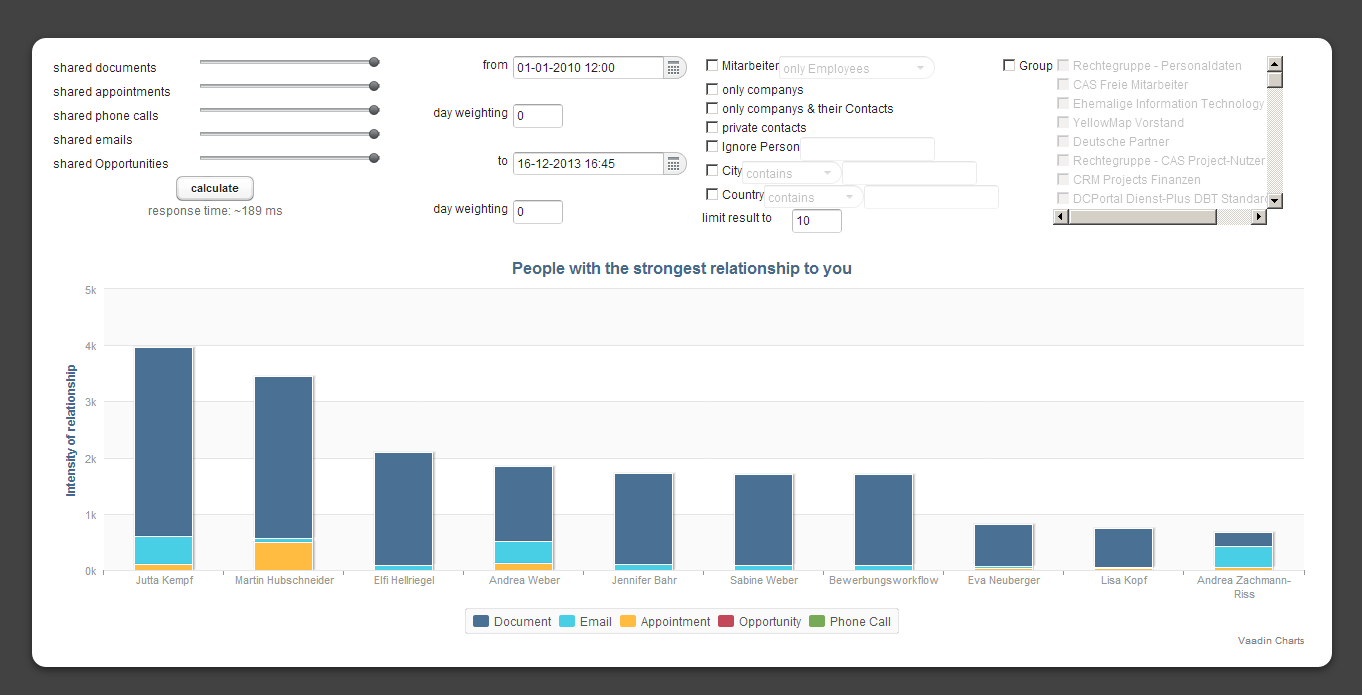
\includegraphics[width=\textwidth]{pics/final_screen.png}
\caption{Oberfläche des Systems}
\label{ergebniss_oberflaeche_haupt}
\end{figure}

Den zentrale Bereich des Fensters stellt das Diagramm dar. Die Balken selbst sind fünf verschiedene Elemente unterteilt. Jedes Elemente wird dabei durch eine andere Farbe dargestellt. Die fünf Elemente sind die verschiedenen Merkmale. Die Zuordnung der Farbe zu dem jeweiligen Merkmal wird über eine Legende im unteren Bereich des Fensters umgesetzt. Eine Besonderheit ist, dass durch einen Klick auf eine der Farben, das jeweilige Merkmal von der Darstellung ausgeschlossen wird. Beispielsweise kann der Nutzer auf die blaue Farbe neben dem Dokument klicken, was einen Neuaufbau des Diagramms, ohne dieses Merkmal bewirkt. Durch diesen Ausschluss wird allerdings keine neue Abfrage gesendet. Das  bedeutet die Reihenfolge in der Personen angezeigt werden bleibt gleich, sowie die Datenbasis. Mit einem wiederholten Klick lässt sich das ganze Rückganggig machen. Zusätzlich zu der Y-Achse, die eine Gesamtpunktzahl aufzeigt, kann der jeweilige Anteil eines Merkmals betrachtet werden. Dies geschieht durch einfaches platzieren des Mauszeigers auf dem jeweiligen Bereich des Balkens. Dadurch öffnet sich ein Tooltip welches die Anzahl der Punkte im Verhältnis zur Gesamtpunktzahl zeigt.

Die Anfragestellung erfolgt in der Regel mit dem dafür vorgesehen Button. Die Regler und das Datum lösen jedoch bei Veränderungen automatisch eine neue Abfrage aus. Dies soll die  die hohe Antwortgeschwindigkeit des Systems untermalen. Das Datum sowie die Gewichtung wurden dafür ausgewählt da diese die am meist benutzen Konfigurationsmöglichkeiten darstellen.